\documentclass[letterpaper,12pt,fleqn]{article}
\usepackage{matharticle}
\usepackage{siunitx}
\usepackage{tikz}
\pagestyle{plain}
\begin{document}

\begin{center}
  \large
  Math-19 Section 1

  \Large
  Homework \#2

  \large
  \textbf{Due: 6/17/2019 9:00am}
\end{center}

\subsection*{Reading}

Sections 1.5 and 1.7

\subsection*{Problems}

\begin{enumerate}
\item A man stands atop a \SI{256}{ft} cliff with a  ball.  Recall that the equation of motion that we presented in
  class is given by:
  \[h=h_0+v_0t-16t^2\]
  \begin{enumerate}
  \item How long does it take for the ball to hit the ground if he simply releases the ball?

  \item How long does it take for the ball to hit the ground if he throws the ball up with a velocity of \SI{16}{ft/s}?

  \item How long does it take for the ball to hit the ground if he throws the ball down with a velocity of
    \SI{16}{ft/s}? (Hint: no additional calculations are needed).

  \item Assume that a lady is standing on the ground below the cliff and throws a ball up so that it passed the man
    on the cliff at a velocity of \SI{16}{ft/s}.  How long would it be before the ball hits the ground? (Hint: you
    already have all the information that you need).
  \end{enumerate}

\item You are a product manager at an electronics firm in charge of a proposed new line of 25-inch monitors (i.e.,
  the length of the diagonal across the screen is 25 inches):

  \begin{tikzpicture}
    \draw (0,0) rectangle (5,3);
    \draw [dashed] (0,0) -- (5,3);
    \node at (2.5,2.0) {25''};
    \node [above] at (2.5,0) {$\ell$};
    \node [right] at (0,1.5) {$w$};
  \end{tikzpicture}

  You realize that the most appealing ratio for the dimensions of the screen would follow the golden ratio:
  \[\frac{\ell}{w}=\frac{1+\sqrt{5}}{2}\approx1.6=\frac{8}{5}\]

  \begin{enumerate}
  \item Using the estimate of $8/5$, determine the dimensions ($\ell\times w$) for the new monitor. Round each
    dimension to two decimal places.
  \item There needs to be an equal amount of casing around the edges of the screen.  The packaging department
    would like the monitor and casing to have a total area of 400 square inches.

    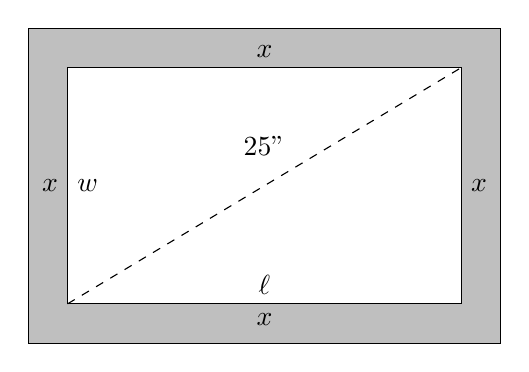
\begin{tikzpicture}
      \draw [fill=lightgray] (-0.5,-0.5) rectangle (5.5,3.5);
      \draw [fill=white] (0,0) rectangle (5,3);
      \draw [dashed] (0,0) -- (5,3);
      \node at (2.5,2.0) {25''};
      \node [above] at (2.5,0) {$\ell$};
      \node [right] at (0,1.5) {$w$};
      \node [above] at (2.5,3) {$x$};
      \node [below] at (2.5,0) {$x$};
      \node [left] at (0,1.5) {$x$};
      \node [right] at (5,1.5) {$x$};
    \end{tikzpicture}

    Determine the width of the casing ($x$) around the screen. Round your answer to
    two decimal places.
  \end{enumerate}
\end{enumerate}

\end{document}
